%%%%%%%%%%%%%%%%%%%%%%%%%%%%%%%%%%%%%%%%%%%%%%%%%%%%%%%%%%%%%%%%%%%%%%%%%%%%%%%%%%%%%%%%%%%%%%%%%%%%
%%%%%%%%%%%%%%%%%%%%%%%%%%%%%%%%%%%%%%%%%%%%%%%%%%%%%%%%%%%%%%%%%%%%%%%%%%%%%%%%%%%%%%%%%%%%%%%%%%%%
%%%%%%%%%%%%%%%%%%%%%%%%%%%%%%%%%%%%%%%%%%%%%%%%%%%%%%%%%%%%%%%%%%%%%%%%%%%%%%%%%%%%%%%%%%%%%%%%%%%%

\subsection{Objective-C et Xcode}

Objective-C est un langage de programmation orienté objet et réflexif.
Compilé et libre, il hérite du langage C (comme le C++) en lui rajoutant l'aspect objet, ce qui lui permet d'être interfacé avec du Langage C ou du C++.
Principalement présent sur les systèmes d'exploitation des produits de la marque Apple (OS X et iOS), ce langage est multi-plateforme.
\\


Xcode est l'environnement de développement intégré (EDI, ou IDE pour Integrated Development Environment) pour Mac OS X.
Il permet le développement d'application en Langage C, C++ et bien évidemment en Objective-C pour OS X ou iOS.
C'est un IDE très complet qui comporte un éditeur de texte, un débogueur, un compilateur, un gestionnaire de projet et de version, un gestionnaire de documents pour la documentation, et d'autres outils facilitant le développement.
\\



%%%%%%%%%%%%%%%%%%%%%%%%%%%%%%%%%%%%%%%%%%%%%%%%%%%%%%%%%%%%%%%%%%%%%%%%%%%%%%%%%%%%%%%%%%%%%%%%%%%%
%%%%%%%%%%%%%%%%%%%%%%%%%%%%%%%%%%%%%%%%%%%%%%%%%%%%%%%%%%%%%%%%%%%%%%%%%%%%%%%%%%%%%%%%%%%%%%%%%%%%
%%%%%%%%%%%%%%%%%%%%%%%%%%%%%%%%%%%%%%%%%%%%%%%%%%%%%%%%%%%%%%%%%%%%%%%%%%%%%%%%%%%%%%%%%%%%%%%%%%%%

\subsection{Les frameworks}

Un \textit{framework} est un ensemble d'outils et de composants structurels qui permettent le développement de logiciels ou de sites web.

Apple propose de nombreux frameworks permettant de simplifier la tâche des développeurs.
Ils respectent les \textit{design patterns} pour structurer l'agencement des différents objets, comme par exemple l'architecture MVC des interfaces graphiques.
Ces frameworks font la force des applications iOS car ils permettent d'interagir très facilement avec les composants des terminaux, comme par exemple le gyroscope, l'appareil photo, l'envoi de mail, l'affichage d'une carte, ...
\\


Il existe deux types de frameworks : les frameworks dits public et les frameworks dits privés.

Les frameworks \textit{publics} doivent être documentés et approuvés par Apple pour que les applications qui les utilisent puissent être publiable sur l'Apple Store.
Cette politique très ferme d'Apple permet d'éviter toute faille de sécurité dans le système et permet de proposer des applications sûres aux utilisateurs.

Les frameworks \textit{privés} proposent des outils de bas niveau non-documentés.
Apple en disposent de plusieurs dans leur kit de développement mais ceux-ci ne peuvent pas être directement utilisés : il est nécessaire d'importer "à la main" des fichiers d'entête (headers ".h") pour pouvoir compiler le projet.
\\



%%%%%%%%%%%%%%%%%%%%%%%%%%%%%%%%%%%%%%%%%%%%%%%%%%%%%%%%%%%%%%%%%%%%%%%%%%%%%%%%%%%%%%%%%%%%%%%%%%%%
%%%%%%%%%%%%%%%%%%%%%%%%%%%%%%%%%%%%%%%%%%%%%%%%%%%%%%%%%%%%%%%%%%%%%%%%%%%%%%%%%%%%%%%%%%%%%%%%%%%%
%%%%%%%%%%%%%%%%%%%%%%%%%%%%%%%%%%%%%%%%%%%%%%%%%%%%%%%%%%%%%%%%%%%%%%%%%%%%%%%%%%%%%%%%%%%%%%%%%%%%

\subsection{Manipulation des SMS}

%%%%%%%%%%%%%%%%%%%%%%%%%%%%%%%%%%%%%%%%%%%%%%%%%%%%%%%%%%%%%%%%%%%%%%%%%%%%%%%%%%%%%%%%%%%%%%%%%%%%

\subsubsection{Envoi de SMS}

Apple n'autorise l'envoi de SMS qu'en utilisant leur framework officiel \textit{MessageUI}.
Lorsque l'application désire envoyer le SMS une fenêtre s'affiche et l'utilisateur doit confirmer l'envoi en appuyant sur le bouton prévu à cet effet.
Cette méthode ne peut pas être utilisée dans ce projet, car l'application mobile fonctionne en tâche de fond et doit envoyer les SMS de manière automatique.

Cependant l'utilisation du framework privé \textit{CoreTelephony} le permet.
L'envoi de SMS peut ainsi se faire grâce à une ligne de code et de manière totalement automatique.
\\

%%%%%%%%%%%%%%%%%%%%%%%%%%%%%%%%%%%%%%%%%%%%%%%%%%%%%%%%%%%%%%%%%%%%%%%%%%%%%%%%%%%%%%%%%%%%%%%%%%%%

\subsubsection{Réception de SMS}

La réception des SMS se décomposent en deux étapes : l'événement de réception, puis la lecture.

\paragraph{Événement de réception -}
Le système envoie des notifications lors des appels ou de la réception des SMS.
Pour que notre programme reçoive ces notifications il est nécessaire de définir une fonction qui sera appelée lorsque ces événements seront émis.
Cela se fait grâce à la fonction \lstinline{CTTelephonyCenterAddObserver()} dans laquelle un des paramètres correspond à la fonction appelée.

% TODO: jailbreak ?


\paragraph{Lecture des SMS -}
Les SMS sont stockés dans une base de données SQLite dont le fichier est \lstinline{/private/var/mobile/Library/SMS/sms.db} dans le répertoire du terminal.
Pour parcourir les messages il est nécessaire d'effectuer des requêtes SQL, comme dans n'importe quelle base de données.

Mais un problème critique : il est impossible d'accéder à ce fichier depuis une application.
En effet, chaque application iOS fonctionne séparément dans sa \textit{sandbox}, qui est un environnement virtuel clos permettant la protection contre les processus malveillants.
Le schéma \ref{iOS_sandbox} représente les différents répertoires des sandbox.
\begin{figure}[!h]
	\center
	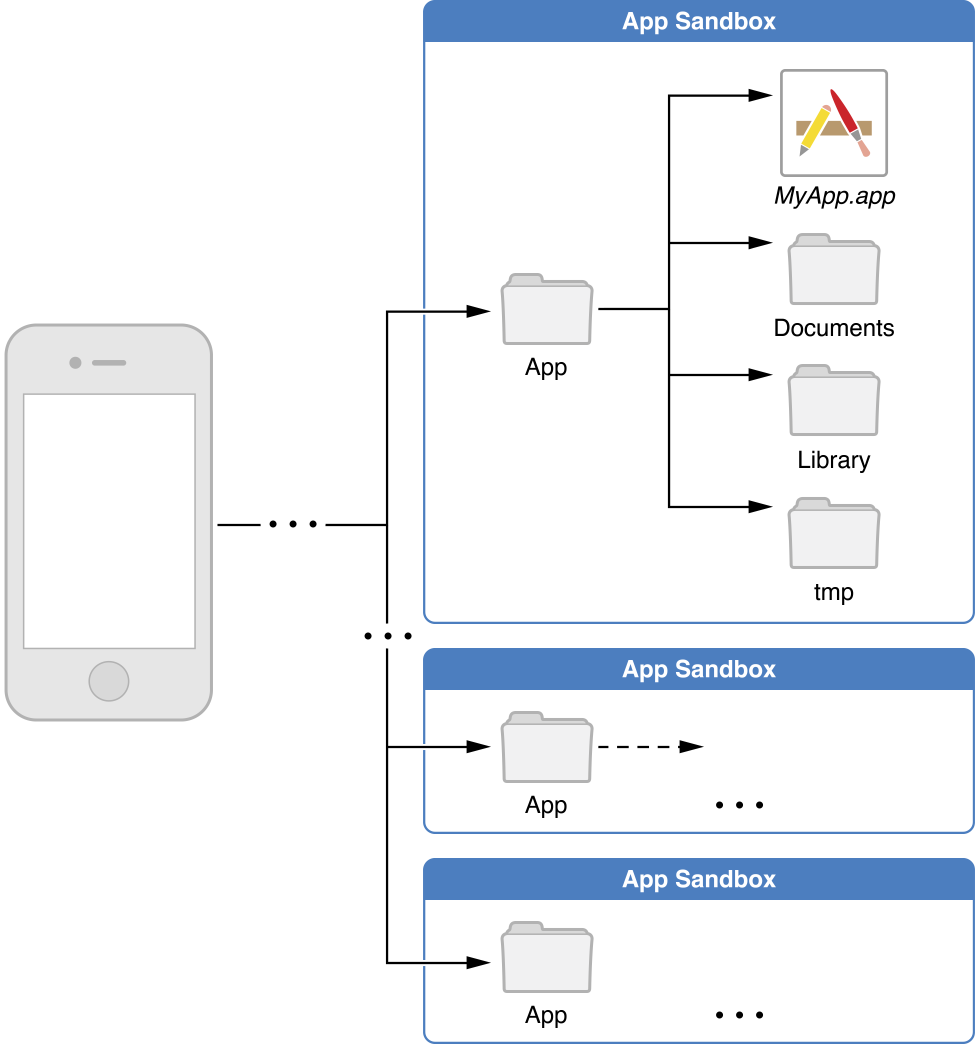
\includegraphics[width=0.4\textwidth]{img/iOS_sandbox.png}
	\caption{Sandbox sous iOS}
	Source : \href{http://developer.apple.com/library/ios/#documentation/iphone/conceptual/iphoneosprogrammingguide/TheiOSEnvironment/TheiOSEnvironment.html}{http://developer.apple.com}
	\label{iOS_sandbox}
\end{figure}

Malheureusement aucune solution d'accès au fichier n'a été trouvée pour le moment.
En attendant de trouver une solution, nous avons copié le fichier dans un répertoire accessible pour effectuer les différents tests de lecture, et la fonction permettant la lecture des SMS renvoie des données "statiques" pour valider le fonctionnement de l'application.
\\



%%%%%%%%%%%%%%%%%%%%%%%%%%%%%%%%%%%%%%%%%%%%%%%%%%%%%%%%%%%%%%%%%%%%%%%%%%%%%%%%%%%%%%%%%%%%%%%%%%%%
%%%%%%%%%%%%%%%%%%%%%%%%%%%%%%%%%%%%%%%%%%%%%%%%%%%%%%%%%%%%%%%%%%%%%%%%%%%%%%%%%%%%%%%%%%%%%%%%%%%%
%%%%%%%%%%%%%%%%%%%%%%%%%%%%%%%%%%%%%%%%%%%%%%%%%%%%%%%%%%%%%%%%%%%%%%%%%%%%%%%%%%%%%%%%%%%%%%%%%%%%

\subsection{Les messages XMPP}

Pour communiquer avec le site internet, le client XMPP de l'application a été développé grâce à \textit{XMPPFramework}\footnote{Source : \href{https://github.com/robbiehanson/XMPPFramework}{https://github.com/robbiehanson/XMPPFramework}}.
Il s'agit d'un framework libre et open-source développé et maintenu par principalement Robbie Hanson.
XMPPFramework est développé en Objective-C destiné aux applications OS X ou iOS.
\\


% TODO: mise en commun avec Androïd ?
Le client XMPP fonctionne comme celui sous Androïd.
Lors de la réception d'un SMS l'application va formater le message sous le format JSON plus envoyer un message XMPP au propre compte Google.
Lors de la réception de messages XMPP l'application va récupérer les données stockées sous le format XMPP puis va envoyer le SMS.
\\


Dans l'application mobile nous n'utiliserons qu'un seul client XMPP et nous voulions qu'il persiste durant toute la vie de l'application (jusqu'à ce que l'utilisateur tue le processus).
Le patron de conception (design pattern) \textit{singleton} a donc été utilisé dans le projet iOS.
En effet singleton permet de s'assurer de n'avoir qu'une seule instance qui persiste en mémoire, et qui de plus est accessible dans toute l'application.
Le schéma \ref{pattern_singleton} représente le diagramme de classe du singleton.
\begin{figure}[!h]
	\center
	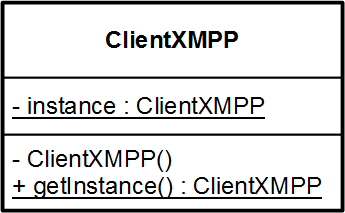
\includegraphics[width=0.3\textwidth]{img/pattern_singleton.png}
	\caption{Pattern singleton : diagramme de classe}
	\label{pattern_singleton}
\end{figure}
~~\\
